\documentclass[10pt,a4paper]{article}
\usepackage[utf8]{inputenc}\usepackage[T1]{fontenc}\usepackage[spanish,es-nodecimaldot]{babel}
\usepackage[margin=2cm]{geometry}\usepackage{tgpagella}\usepackage{graphicx,booktabs,xcolor,titlesec,enumitem}
\definecolor{Inst}{HTML}{3B4674}\titleformat{\section}{\large\bfseries\color{Inst}}{}{0pt}{}[\vspace{-4pt}\titlerule]
\pagestyle{empty}\setlength{\parindent}{0pt}\setlist{nosep,leftmargin=*}
\begin{document}
{\LARGE\bfseries\color{Inst} Cubicación de obra gruesa}\\[2pt]
{\large Vivienda de un piso, 59.4 m\textsuperscript{2} \hfill Muestra de trabajo}\\[2pt]
Nicolás Albornoz Pavez \textbullet{} Estudiante de Ingeniería Civil, UTFSM \hfill 16 de noviembre de 2026

\section{Planta medida}
\begin{center}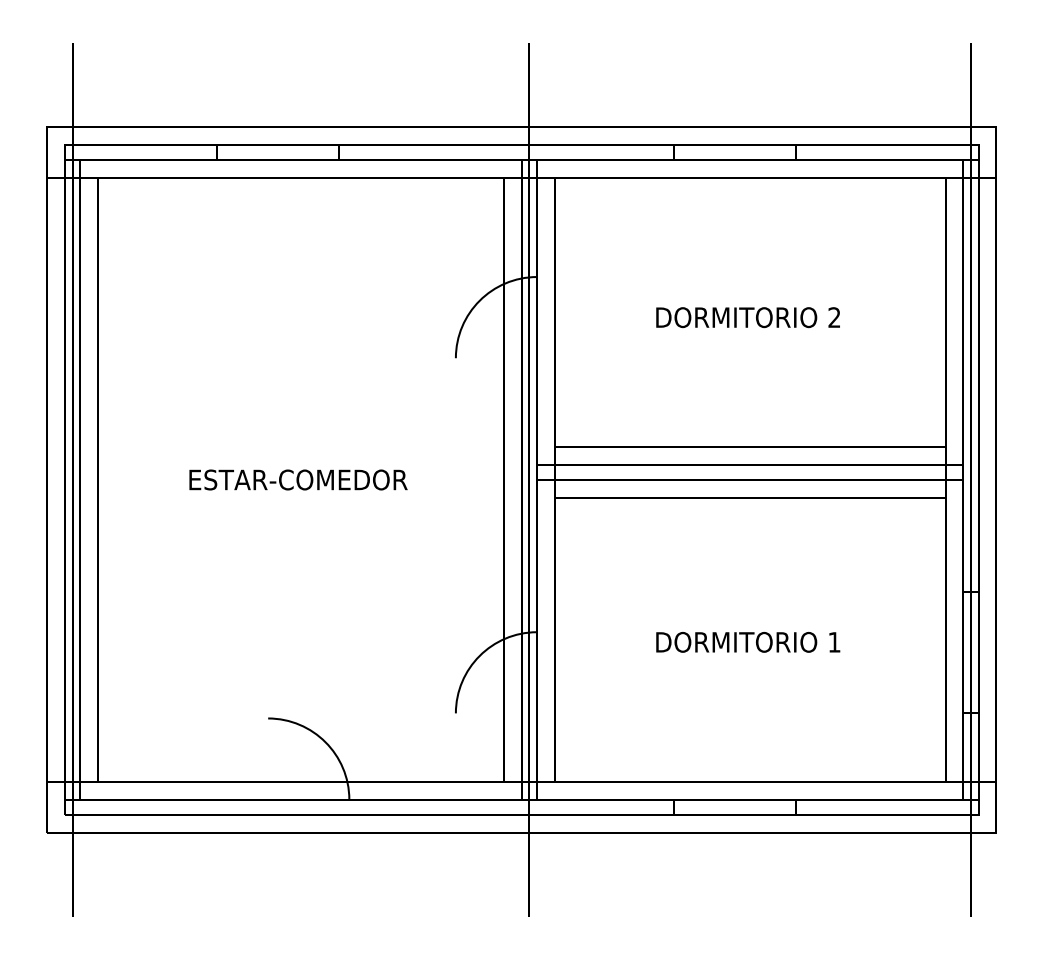
\includegraphics[width=0.62\textwidth]{planta.png}\end{center}
Plano propio en formato DXF, dibujado en milímetros. Capas medidas: fundaciones, muros, radier y vanos.

\section{Cantidades}
\begin{tabular*}{\textwidth}{@{\extracolsep{\fill}}llcrrr@{}}\toprule
Ítem & Partida & Unidad & Cantidad neta & Pérdida & Cantidad final\\\midrule
1.1 & Excavación de zanjas para fundación & m\textsuperscript{3} & 12.12 & 0 \% & 12.12\\
1.2 & Hormigón de fundación corrida & m\textsuperscript{3} & 12.12 & 5 \% & 12.73\\
2.1 & Radier $e = 10$ cm, superficie & m\textsuperscript{2} & 53.24 & 0 \% & 53.24\\
2.2 & Hormigón de radier & m\textsuperscript{3} & 5.32 & 3 \% & 5.48\\
3.1 & Muros de albañilería $e = 15$ cm & m\textsuperscript{2} & 89.04 & 5 \% & 93.49\\
4.1 & Puertas de 0.80 $\times$ 2.00 m & un & 3 & -- & 3\\
4.2 & Ventanas de 1.20 $\times$ 1.00 m & un & 4 & -- & 4\\\bottomrule
\end{tabular*}

\section{Método y control}
Las cantidades se extraen por capa desde el DXF con un script propio en Python, probado contra geometrías de resultado conocido, y se contrastan con un segundo cálculo independiente por dimensiones.

\medskip
\begin{tabular*}{\textwidth}{@{\extracolsep{\fill}}lrrr@{}}\toprule
Elemento & Script & Cálculo por dimensiones & Diferencia\\\midrule
Fundaciones, área en planta [m\textsuperscript{2}] & 20.200 & $40.4 \times 0.50 = 20.200$ & 0.0 \%\\
Radier [m\textsuperscript{2}] & 53.235 & $4.35\times6.30 + 4.20\times3.15 + 4.20\times3.00 = 53.235$ & 0.0 \%\\
Muros, área en planta [m\textsuperscript{2}] & 6.165 & $41.1 \times 0.15 = 6.165$ & 0.0 \%\\\bottomrule
\end{tabular*}

\section{Supuestos y exclusiones}
\begin{itemize}
\item Altura de fundación 0.60 m, altura de muro 2.40 m y espesor de radier 0.10 m; el plano es solo de planta.
\item Descuento de vanos en muros: $3 \times 0.80 \times 2.00 + 4 \times 1.20 \times 1.00 = 9.60$ m\textsuperscript{2}.
\item No incluye enfierradura, moldajes, techumbre, terminaciones ni precios.
\item Cubicación referencial elaborada desde el plano indicado. No reemplaza un proyecto ni un presupuesto firmado por un profesional competente.
\end{itemize}
\end{document}
